		\section{Динамика пополнения поселений {\it Macoma balthica} в Белом море}
При изучении динамики поселений бентосных организмов с планктонной личинкой важную роль играет пополнение поселений молодью. 
Оседание {\it M.~balthica} в Белом море происходит с июля по сентябрь (\cite{Semenova_1980, Maximovich_1985}), поэтому данные, собранные в июле, не описывают величину оседания в текущем году. 
Однако мы можем оценить пополнение предыдущего года по обилию особей возрастом 1+. 
Для Северного моря показано, что в пополнении поселений молодью выживаемость спата в первую зиму не менее важна, чем непоследственно количество осевших особей (\cite{Beukema_et_al_1998, Strasser_Gunter_2001}). Подобные данные известны и для Белого моря (\cite{Maximovich_Gerasimova_2004}). Поэтому, на наш взгляд, с точки зрения существования поселения, оценка пополнения поселения как численности особей, переживших первую зиму, более информативна.




	\subsection{Размер моллюсков {\it M.~balthica} в возрасте 1 года}

Поскольку в мониторинговых исследованиях в вершине Кандалакшского залива фиксировалась только длина раковины без определения возраста, то в $2012 - 2013$ году были проведены  измерения длин колец зимней остановки роста у особей длиной менее $3$~мм (рис. \ref{ris:vozrast_menee_3mm}, A). 
Данные получены для участков на о.~Горелый, в эстуарии р.~Лувеньги и в Западной Ряшковой салме. 
Распределение измереных особей по возрастам представлено на рис. \ref{ris:vozrast_menee_3mm}, B.
	\begin{figure}[hbp]
		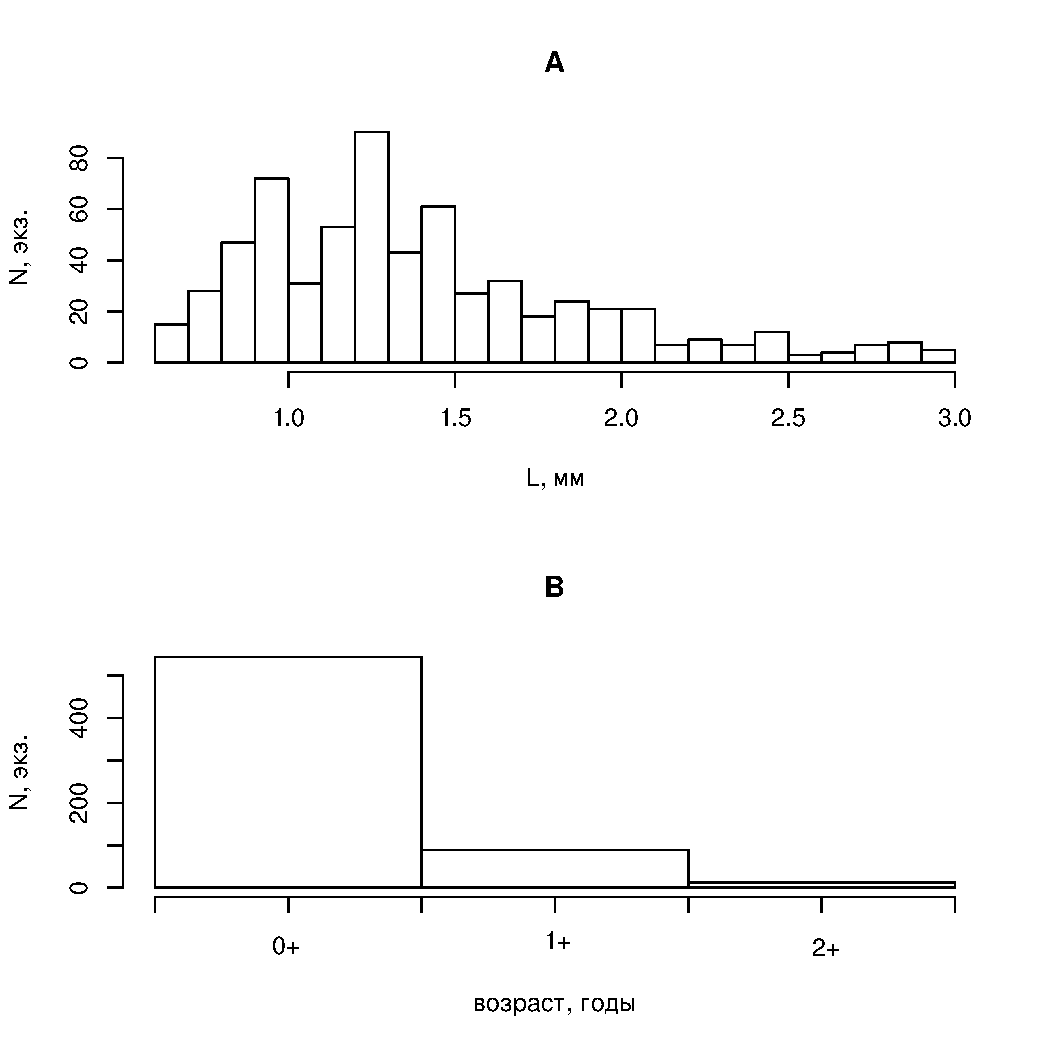
\includegraphics{../White_Sea/growth_young/hist_obili_po_godam1.pdf}
	\caption{Распределение моллюсков {\it M.~balthica} длиной менее $3$~см по размеру (А) и возрасту (В)}
	\label{ris:vozrast_menee_3mm}
	{\footnotesize Примечание: N, экз. \textemdash количество особей, L, мм \textemdash длина раковины}
	\end{figure}

Особи возрастом 1+ с различных горизонтов литорали острова Горелый не различаются по размеру ($Kruskal-Wallis\ \chi^2 = 3,12, p = 0,37$), поэтому в дальнейшем мы рассматриваем их как одну выборку (рис. \ref{ris:Goreliy_length1+_gorizonty}).
	\begin{figure}[hbp]
		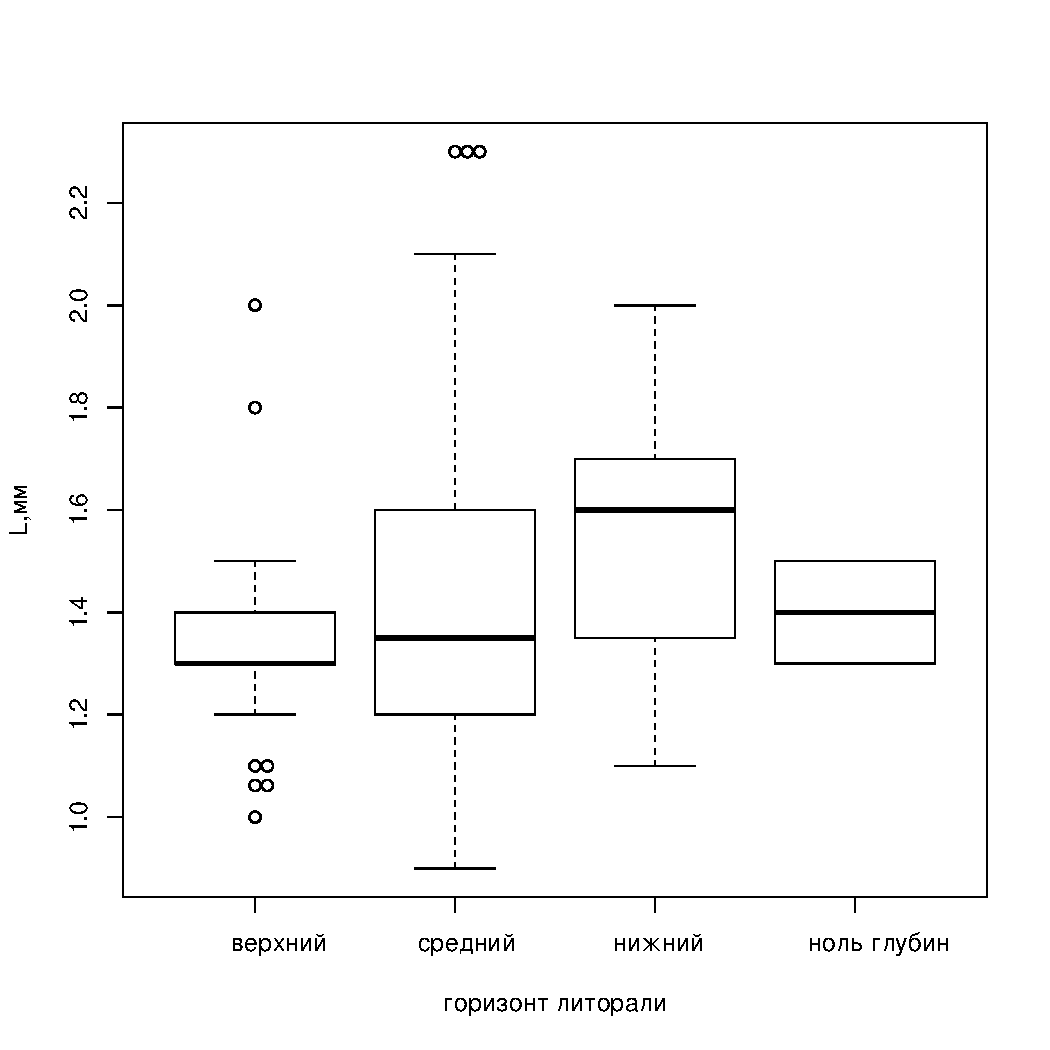
\includegraphics{../White_Sea/growth_young/boxplot_Goreliy_length_1+_tidal.pdf}
	\caption{Размеры  годовалых моллюсков {\it M.~balthica} на разных горизонтах литорали о. Горелый}
	\label{ris:Goreliy_length1+_gorizonty}
	{\footnotesize Примечание: L, мм \textemdash длина раковины. <<Ящик>> на графике соответствует 1 и 3 квартилю, жирная горизонтальная линия \textemdash 		медиана, <<усы>> \textemdash $1,5$ межквартильных размаха}
	\end{figure}

По результатам теста Краскел-Уоллиса годовалые моллюски с разных участков различались по длине ($Kruskal-Wallis\ \chi^2 = 17,6, p = 0,00015$) (\ref{ris:length_1+_uchastki}, поэтому было проведено попарное сравнение участков (табл.~\ref{tab:Tukey_1+_uchastki}). 
Размер годовалых особей не различался на участках, расположенных в районе Лувеньгиских шхер (о.~Горелый и эстуарий р.~Лувеньги), и отличался от особей из Западной Ряшковой салмы.
	\begin{figure}[hbp]
		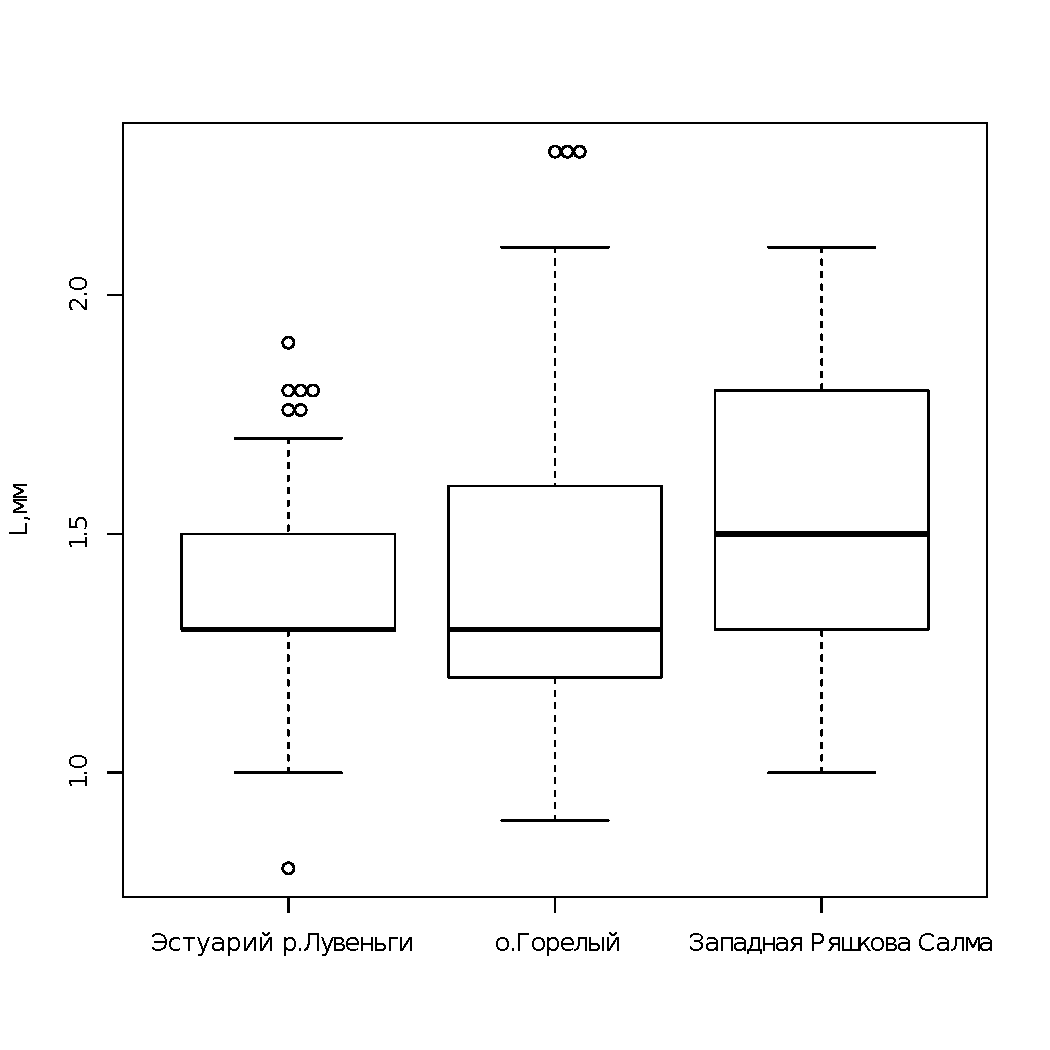
\includegraphics{../White_Sea/growth_young/boxplot_length_1age_area1.pdf}
	\caption{Размеры  годовалых моллюсков {\it M.~balthica} на разных участках литорали}
	\label{ris:length_1+_uchastki}
	{\footnotesize Примечание: L, мм \textemdash длина раковины. <<Ящик>> на графике соответствует 1 и 3 квартилю, жирная горизонтальная линия \textemdash 		медиана, <<усы>> \textemdash $1,5$ межквартильных размаха}
	\end{figure}
	
	\begin{table}[hbp]
	\begin{tabular}{|*{4}{p{0.2\textwidth}|}} \hline
	участки & различия средних & p-value & достоверность различий\\
	\hline
	о.~Горелый \textemdash\ эстуарий р.~Лувеньги & $0,053$ & $0,2$ & \\
	\hline
	о.~Горелый \textemdash\ Западная Ряшкова салма & $0,11$ & $0,005$ & ** \\
	\hline
	эстуарий р.~Лувеньги \textemdash\ Западная Ряшкова салма & $0,17$ & $0.00002$ & ***\\
	\hline
	\end{tabular}
	
	{\footnotesize Примечание: достоверность различий *** \textemdash $p<0,001$; ** \textemdash $p<0,05$; * \textemdash $p<0,1$.}
	\caption{Результаты множественного сравнения длины годовалых {\it Macoma balthica} на различных участках методом Тьюки (Tukey's ‘Honest Significant Difference’).}
	\label{tab:Tukey_1+_uchastki}
	\end{table}

Для определения границ размерно-возрастных классов {\it Macoma balthica} возрастом $0+$, $1+$ и $2+$ были рассчитаны средние размеры особей каждого возраста (табл~\ref{tab:mean_length_ages}).
	\begin{table}[hbp]
	\begin{tabular}{|l|*{3}{p{0.2\textwidth}|}} \hline
	возраст & $0+$ & $1+$ & $2+$\\
	\hline
	о.~Горелый & $1,0 \pm 0,001$ & $1,4 \pm 0,002$ & $2,2 \pm 0,008$ \\ 
	\hline
	эстуарий р.~Лувеньги & $1,0 \pm 0,004$ & $1,4 \pm 0,002$ & $2,2 \pm 0,02$ \\
	\hline
	Западная Ряшкова салма & $1,1 \pm 0,04$ & $1,5 \pm 0,003$ & $2,3 \pm 0,02$ \\ 
	\hline
	\end{tabular}
	
	{\footnotesize Примечание: В ячейках указано среднее арифметическое с ошибкой.}
	\caption{Средний размер {\it Macoma balthica}в возрасте до 2 лет на различных участках.}
	\label{tab:mean_length_ages}
	\end{table}
Пограничный размер между двумя когортами рассчитывали как середину между средними размерами особей в когорте. 
Таким образом, в дальнейшем для участков, расположенных в акватории Лувеньгских шхер, маком длиной менее $1,2$~мм рассматривали как спат, а длиной от $1,2$ до $1,8$~мм \textemdash\ как особей возрастом 1+.
Для участков на о.~Ряшков пограничные значения составили $1,3$ и $1,9$,~мм соответственно.
Для участка на о.Ломнишном мы использовали данные, полученные для о.~Ряшкова.





\par\bigskip

Таким образом были получены данные по динамике численности годовалых маком на 6 мониторинговых участок (рис.~\ref{ris:dynamic_1year_Kandalaksha}).
	\begin{figure}[p]
	
	\begin{minipage}[b]{.46\linewidth}
	%Фигурка в первом ряду слева размер отведенный под весь этот объект \textendash 0.46 от ширины строки
	%Параметр [b] означает, что выравнивание этих министраниц будет по нижнему краю
	\begin{center}
	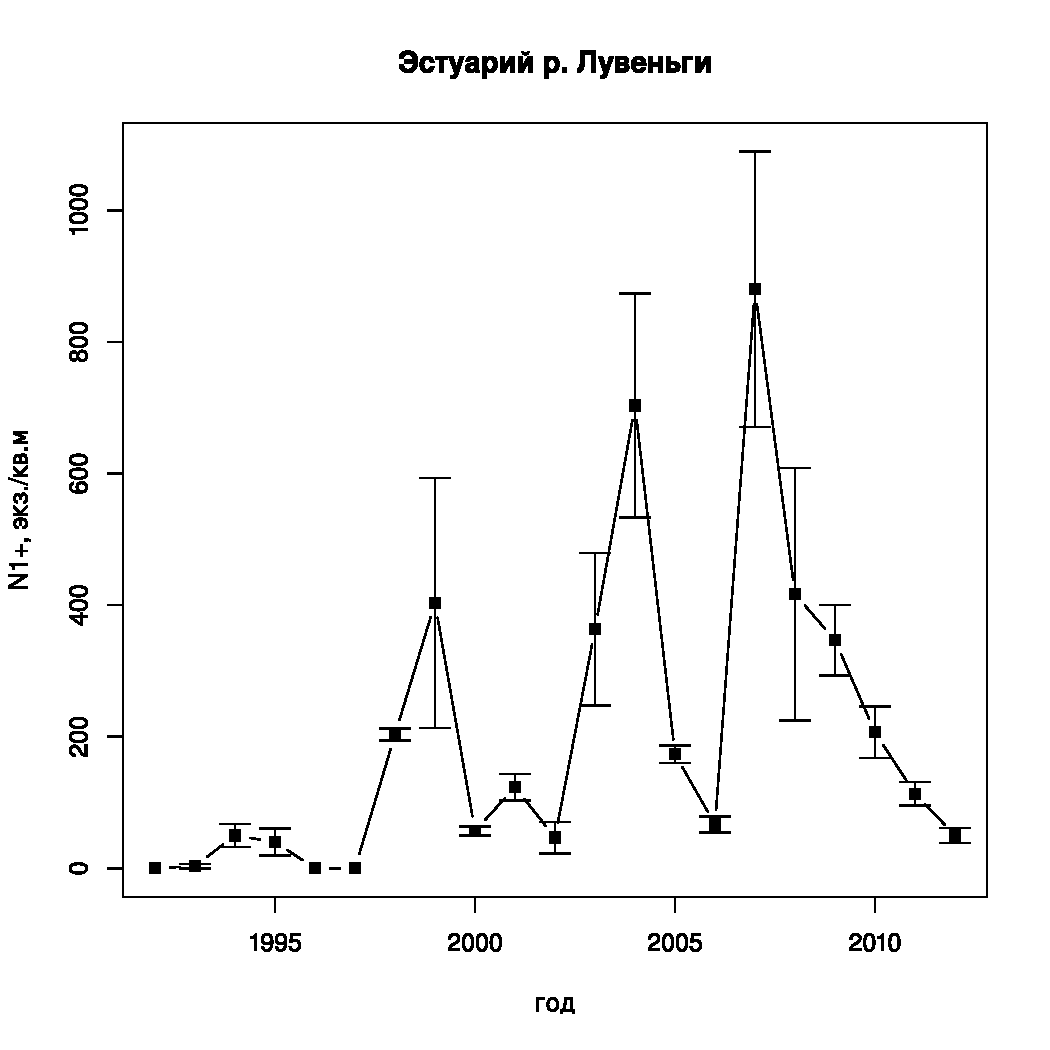
\includegraphics[width=65mm]{../White_Sea/Estuatiy_Luvenga/Estuary_N_oneyear1.pdf}

	\end{center}
	\end{minipage}
	%
	\hfil %Это пружинка отодвигающая рисунки друг от друга
	%
	\begin{minipage}[b]{.46\linewidth}
%Следующий рисунок - первый ряд справа %DUNGEON S_4 \ AB
	\begin{center}
		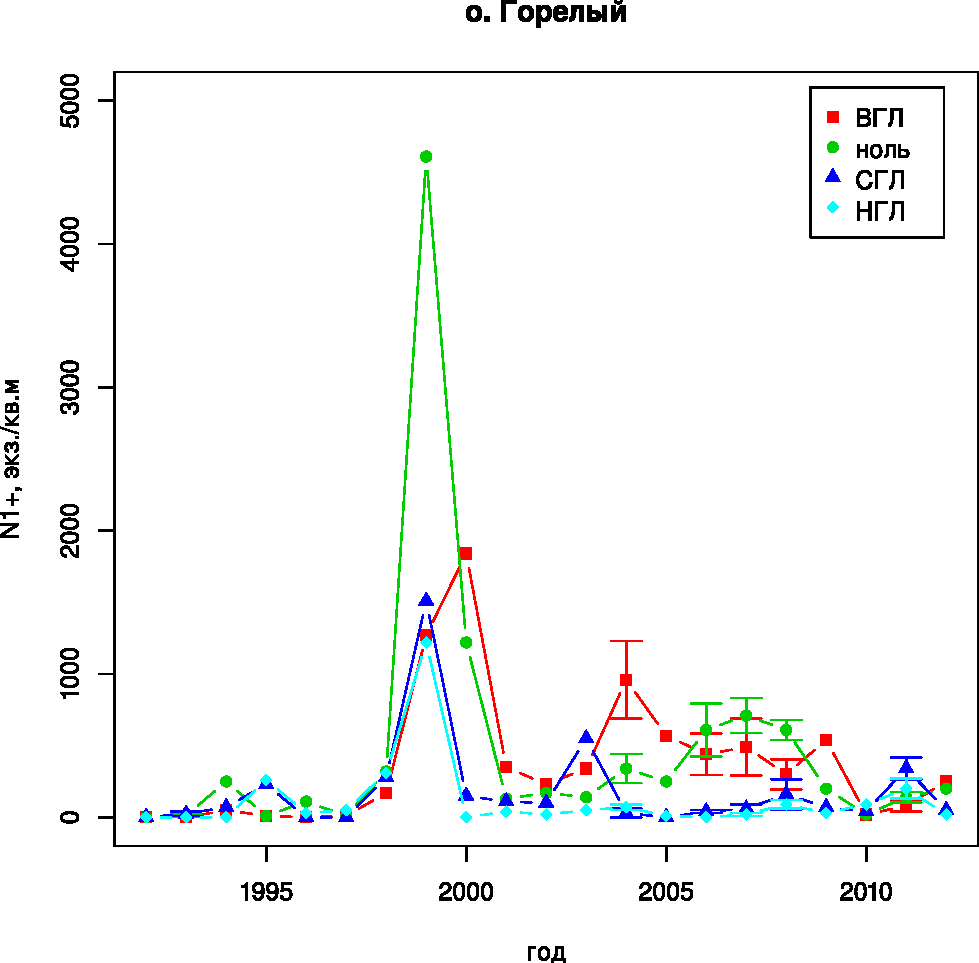
\includegraphics[width=65mm]{../White_Sea/Luvenga_Goreliy/Goreliy_N_oneyear1.pdf}
	\end{center}
	\end{minipage}

%\smallskip


	\begin{minipage}[b]{.46\linewidth}
%Фигурка в первом ряду слева размер отведенный под весь этот объект \textendash 0.46 от ширины строки
%Параметр [b] означает, что выравнивание этих министраниц будет по нижнему краю
	\begin{center}
		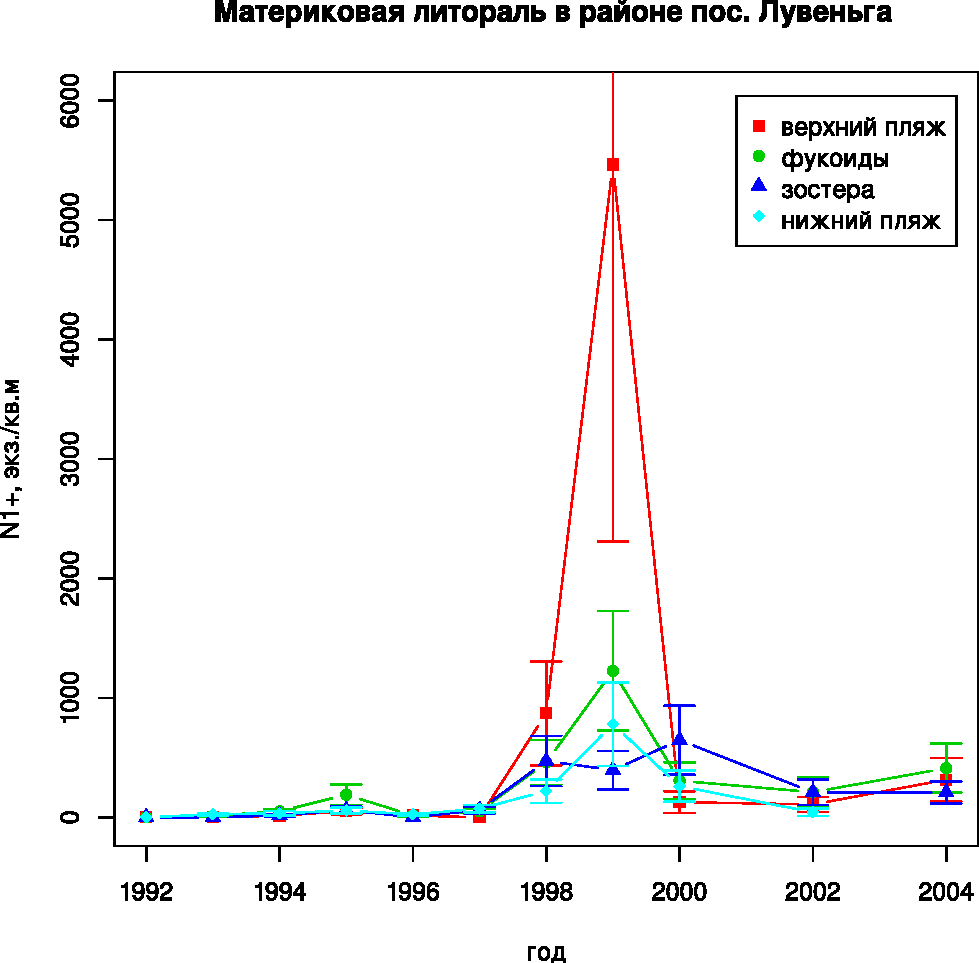
\includegraphics[width=65mm]{../White_Sea/Luvenga_II_razrez/2razrez_N_oneyear1.pdf}
	\end{center}
	\end{minipage}
%
	\hfil %Это пружинка отодвигающая рисунки друг от друга
%
	\begin{minipage}[b]{.46\linewidth}
%Следующий рисунок - первый ряд справа %DUNGEON S_4 \ AB
	\begin{center}
		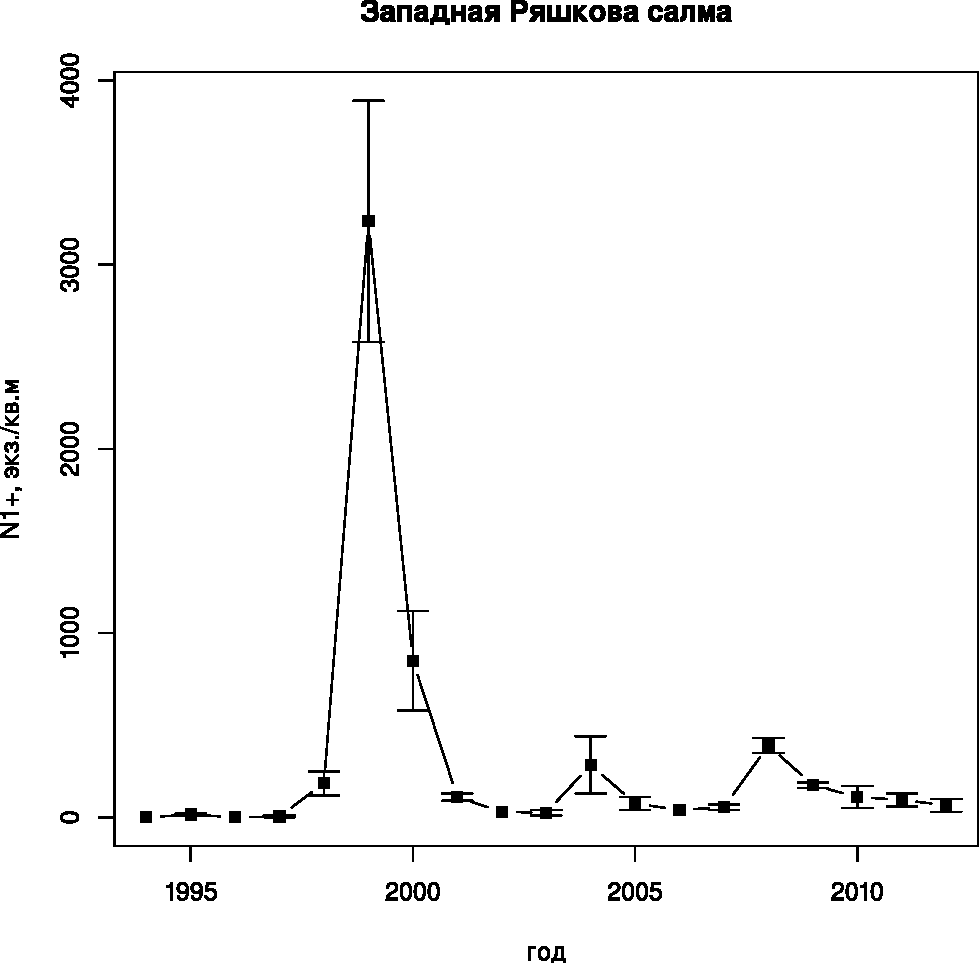
\includegraphics[width=65mm]{../White_Sea/Ryashkov_ZRS/ZRS_N_oneyear1.pdf}
	\end{center}
	\end{minipage}

%\smallskip

	\begin{minipage}[b]{.46\linewidth}
%Фигурка в первом ряду слева размер отведенный под весь этот объект \textendash 0.46 от ширины строки
%Параметр [b] означает, что выравнивание этих министраниц будет по нижнему краю
	\begin{center}
		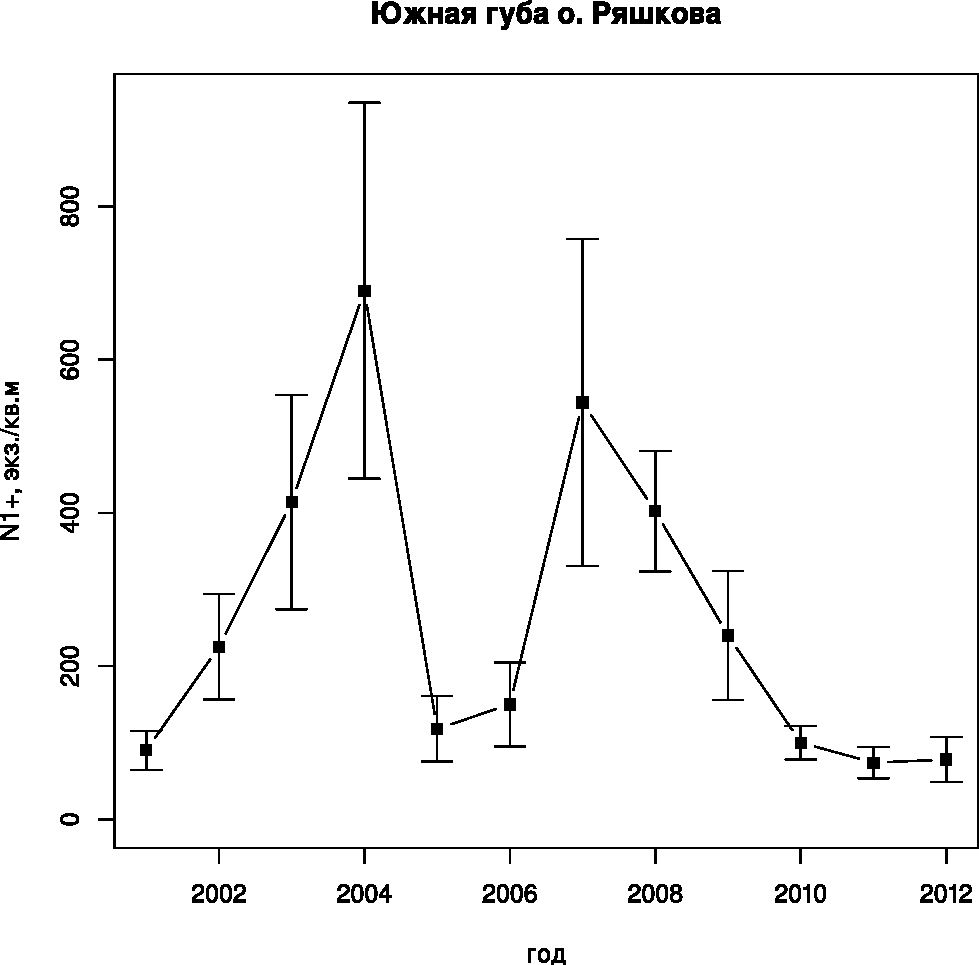
\includegraphics[width=65mm]{../White_Sea/Ryashkov_YuG/YuG_N_oneyear1.pdf}
	\end{center}
	\end{minipage}
%
	\hfil %Это пружинка отодвигающая рисунки друг от друга
%
	\begin{minipage}[b]{.46\linewidth}
%Следующий рисунок - первый ряд справа %DUNGEON S_4 \ AB
	\begin{center}
		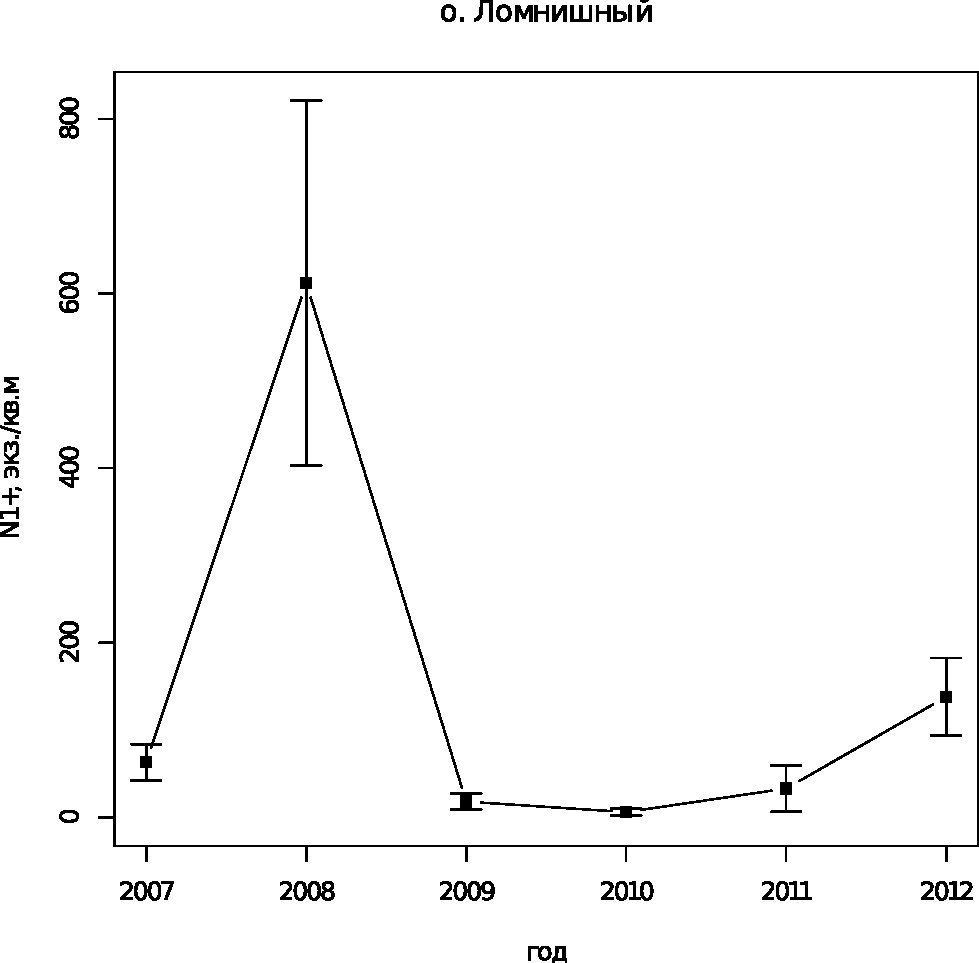
\includegraphics[width=65mm]{../White_Sea/Lomnishniy/Lomnishniy_N_oneyear1.pdf}
	\end{center}
	\end{minipage}

%\smallskip
	\caption{Динамика численности годовалых {\it Macoma balthica} в вершине Кандалакшского залива}
	\label{ris:dynamic_1year_Kandalaksha}
	\end{figure}
Численность годовалых особей знаительно варьирует год от года. 
В некоторые годы макомы возрастом $1+$ отсутствуют в поселениях.
Максимальные численности годовалых особей варьировали между участками от $600$ на Ломнишном до $5500$ на верхнем горизонте материковой литорали в Лувеньге.

Важно отметить, что именно флуктуации численности годовалых особей во-многом определяют изменения общего обилия маком (рис.~\ref{ris:N1year_vs_Nall}).
    \begin{figure}[p]
        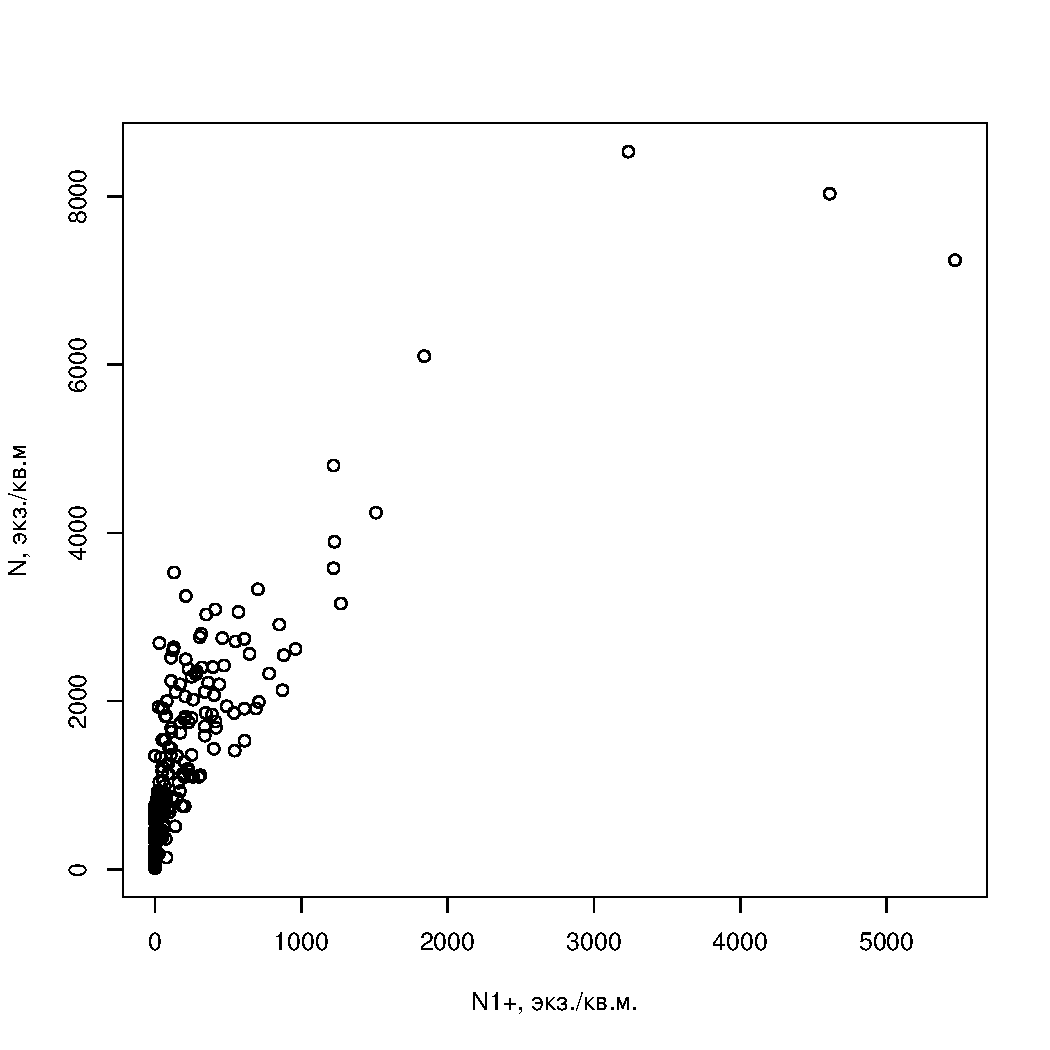
\includegraphics[width=\textwidth]{../White_Sea/oneyear_all_Kandalaksha_all/N1y_vs_N2_1.pdf}
    \caption{Соотношение общей численности {\it Macoma balthica} и численности особей возрастом 1+}
    \label{ris:N1year_vs_Nall}

	\footnotesize{Примечание: N1+ ---численность маком возрастом 1 год, экз./м$^2$. N --- общая численность маком в поселении, экз./м$^2$.}
    \end{figure}
Корреляция между данными параметрами показывает сильную связь ($Spearman\ \rho = 0,83, p < 0,0001$).

Для проверки связи пополнения с численностью половозрелых особей в поселении мы использовали численность маком крупнее $8$~мм, поскольку в Белом море показано (\cite{Semenova_1980, Maximovich_1985}), что ключевым фактором для возможности половозрелости является именно размер (рис.~\ref{ris:N1year_vs_N8mm}).
    \begin{figure}[p]
        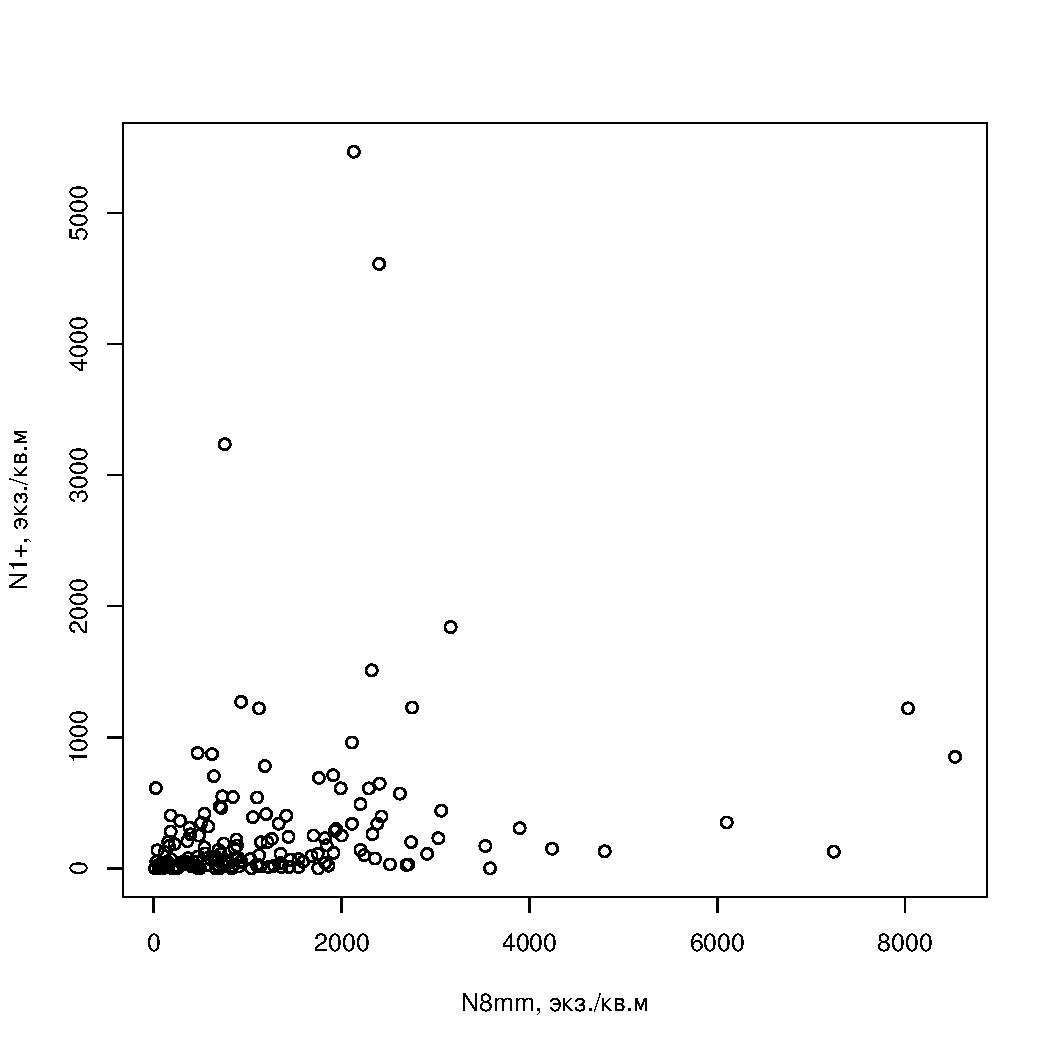
\includegraphics[width=\textwidth]{../White_Sea/oneyear_all_Kandalaksha_all/N8mm_vs_N1y_1.pdf}
    \caption{Связь численность годовалых особей {\it Macoma balthica} и количества половозрелых особей в год их оседания}
    \label{ris:N1year_vs_N8mm}

	\footnotesize{Примечание: N8mm --- численность маком с длиной раковины больше $8$~мм в поселении  в год оседания, экз./м$^2$. N1+ ---численность годовалых маком через год после года оседания, экз./м$^2$.}
    \end{figure}
Коэффициент коллеряции Спирмена между указанными параметрами был достоверный, но низкий ($Spearman\ \rho = 0,39, p < 0,0001$). 

Если при размножении формируется общий личиночный пул, а в дальнейшем на выживаемость влияют зимние условия, можно предположить, что географически близкие поселения должны пополнятся синхронно.
Мы проверили гипотезу о синхронности пополнения поселений при помощи корреляции Мантеля (табл.~\ref{tab:Mantel_dynamic_N1y}).
	\begin{table}[p]
	\caption{Синхронность динамики пополнения поселений {\it Macoma balthica}}
	\label{tab:Mantel_dynamic_N1y}
        \begin{tabularx}{\textwidth}{|p{0.2\textwidth}|*{6}{X|}} 
	\hline
	$Mantel \ r \setminus p_{perm}$ & [1] & [2] & [3] & [4] & [5] & [6] \\ \hline
	[1] Эстуарий р.~Лувеньги             &         & $0,13$    & $0,793$      & $0,118$   & \cellcolor{yellow}{$0,001$} & $0,176$ \\ \hline
	[2] о.~Горелый             & $0,089$   &         & $0,413$      & \cellcolor{yellow}{$0,009$}   & \cellcolor{yellow}{$0,004$} & \cellcolor{yellow}{$0,001$} \\ \hline
	[3] о.~Ломнишный          & $-0,226$  & $-0,003$  &            & NA      & $0,189$ & $0,128$ \\ \hline
	[4] материк (Лувеньга)             & $0,388$   & \cellcolor{yellow}{$0,955$}   & NA         &         & NA    & \cellcolor{yellow}{$0,02$}  \\ \hline
	[5] Южная губа, о.~Ряшков                 & \cellcolor{yellow}{$0,793$}   & \cellcolor{yellow}{$0,515$}   & $0,212$      & NA      &       & $0,12$  \\ \hline
	[6] Западная Ряшкова салма                 & $0,029$   & \cellcolor{yellow}{$0,986$}   & $0,914$      & \cellcolor{yellow}{$0,965$}   & $0,276$ &       \\ \hline 
	\end{tabularx}
	   {\footnotesize Примечание: Нижняя половина таблицы --- значение теста Мантеля, верхняя половина --- уровень значимости, определенный пермутационным методом. \\
	Желтым выделены значения с уровнем значимости $< 0,05$. \\
	$NA$ --- ряды не пересекаются во времени.}
	\end{table}
Синхронность в пополнении была показана для ряда участков.
В поселении на о.~Горелом успешные пополнения происходили синхронно с поселениями на материковой литорали в Лувеньге и двумя участками литорали на о.~Ряшкове (Южная губа и Западная Ряшкова салма).
Также элементы синхронности были отмечены для поселений на о.~Ряшкове с участком в эстуарии р.~Лувеньги.

Также было проведено сравнение степени синхронности динамики пополнения поселений (в качестве меры синхронности использовали значение коэффициента корреляции Мантеля) и расстояния между участками.
Не было показано достоверной связи между указанными параметрами ($Mantel\ r = -0,08, p = 0,67$ ).

